\chapter{Rekurrenz-Gleichungen} 
In diesem Kapitel stellen wir 
Rekurrenz-Gleichungen\footnote{
Rekurrenz-Gleichungen werden in der Literatur auch als \emph{Rekursions-Gleichungen} bezeichnet.}
vor und zeigen, wie diese in einfachen F\"{a}llen gel\"{o}st werden k\"{o}nnen.  
Rekurrenz-Gleichungen treten in der Informatik bei der Analyse der Komplexit\"{a}t von
Algorithmen auf.


\section{Die Fibonacci-Zahlen}
Wir wollen \emph{Rekurrenz-Gleichungen} anhand eines eher spielerischen Beispiels
einf\"{u}hren.  Dazu betrachten wir eine Kaninchen-Farm, f\"{u}r die wir einen Gesch\"{a}ftsplan
erstellen wollen.   Wir besch\"{a}ftigen uns hier nur mit der Frage, wie sich eine
Kaninchen-Population entwickelt.  Wir gehen dabei von folgenden vereinfachenden Annahmen aus:
\begin{enumerate}
\item Jedes Kaninchen-Paar bringt jeden Monat ein neues Kaninchen-Paar zur Welt.
\item Kaninchen haben nach zwei Monaten zum ersten Mal Junge.
\item Kaninchen leben ewig.
\end{enumerate}
Wir nehmen nun an, wir h\"{a}tten ein neugeborenes Kaninchen-Paar und stellen uns die Frage, wie
viele Kaninchen-Paare wir nach $n$ Monaten haben.  Bezeichnen wir die Zahl der
Kaninchen-Paare nach $n$ Monaten mit $k(n)$, so gilt:
\begin{enumerate}
\item $k(0) = 1$

      Wir starten mit einem neugeborenem Kaninchen-Paar.
\item $k(1) = 1$

      Kaninchen bekommen das erste Mal nach zwei Monaten Junge, also hat sich die Zahl
      der Kaninchen-Paare nach einem Monat noch nicht ver\"{a}ndert.
\item $k(2) = 1 + 1$

      Nach zwei Monaten bekommt unser Kaninchen-Paar zum ersten Mal Junge.
\item Allgemein gilt nach $n + 2$ Monaten: \\[0.2cm]
      \hspace*{1.3cm} 
      $k(n+2) = k(n+1) + k(n)$

      Alle Kaninchen-Paare, die zum Zeitpunkt $n$ schon da sind, bekommen zum Zeitpunkt
      $n+2$ Junge. Dies erkl\"{a}rt den Term $k(n)$.  Da wir zur Vereinfachung unserer
      Rechnung von genetisch manipulierten unsterblichen Kaninchen ausgehen, sind alle
      Kaninchen, die zum Zeitpunkt $n+1$ vorhanden sind, auch noch zum Zeitpunkt $n+2$
      vorhanden. Dies erkl\"{a}rt den Term $k(n+1)$. 
\end{enumerate}
Die Folge der Zahlen $\bigl(k(n)\bigr)_{n\in\mathbb{N}}$ ist im Wesentlichen\footnote{
    In der Literatur wird die Folge $(f_n)_{n \in \mathbb{N}}$ der Fibonacci-Zahlen meist
    durch die Gleichungen 
    \\[0.1cm]
    \hspace*{1.3cm}
    $f_0 = 0$, \quad $f_1 = 1$ \quad und \quad $f_{n+2} = f_{n+1} + f_n$
    \\[0.1cm]
    definiert. Dann gilt $k(n) = f_{n+1}$, die Folge $\bigl(k(n)\bigr)_{n \in \mathbb{N}}$
    geht also aus der Folge der Fibonacci-Zahlen $(f_n)_{n \in \mathbb{N}}$ dadurch
    hervor, dass der erste Wert der Folge abgeschnitten wird.
}
 die Folge der
\emph{Fibonacci-Zahlen}.   

Das Programm in Abbildung
\ref{fig:fibonacci} auf Seite \pageref{fig:fibonacci} berechnet diese Zahlen.

\begin{figure}[!h]
  \centering
\begin{Verbatim}[ frame         = lines, 
                  framesep      = 0.3cm, 
                  labelposition = bottomline,
                  numbers       = left,
                  numbersep     = -0.2cm,
                  xleftmargin   = 0.8cm,
                  xrightmargin  = 0.8cm
                ]
    fibonacci := procedure(n) {
        if (n in {0, 1}) {
            return 1;
        }
        return fibonacci(n-1) + fibonacci(n-2);
    };
    
    for (n in [0 .. 100]) {
        print("fibonacci($n$) = $fibonacci(n)$");
    }
\end{Verbatim}
\vspace*{-0.3cm}
  \caption{Ein naives Programm zur Berechnung der Fibonacci-Zahlen.}
  \label{fig:fibonacci}
\end{figure} 

Wenn wir dieses Programm laufen lassen, stellen wir fest, dass die Laufzeiten mit
wachsendem Parameter $n$ sehr schnell anwachsen.  Um dieses Ph\"{a}nomen zu analysieren,
untersuchen wir exemplarisch, wie viele Additionen bei der Berechnung von
$\texttt{fibonacci}(n)$ f\"{u}r ein gegebenes $n \in \mathbb{N}$ ben\"{o}tigt werden.  Bezeichnen wir
diese Zahl mit $a_n$, so finden wir:
\begin{enumerate}
\item $a_0 = 0$.
\item $a_1 = 0$.
\item $n \geq 2 \rightarrow a_n = a_{n-1} + a_{n-2} + 1$,

      denn in den rekursiven Aufrufen $\texttt{fibonacci}(n-1)$ und $\texttt{fibonacci}(n-2)$ haben wir 
      $a_{n-1}$ bzw.~$a_{n-2}$ Additionen und dazu kommt noch die Addition der Werte
      $\texttt{fibonacci}(n-1)$ und $\texttt{fibonacci}(n-2)$.
\end{enumerate}
Wir setzen in der  Gleichung $a_n = 1 + a_{n-1} + a_{n-2}$ f\"{u}r $n$ den Wert $i+2$ ein und
haben dann 
\begin{equation}
  \label{eq:fibonacci1}
 a_{i+2} = a_{i+1} + a_i + 1  
\end{equation}
Eine solche Gleichung nennen wir eine \emph{lineare} \emph{inhomogene}
\emph{Rekur\-renz-Gleichung}.   Die dieser Gleichung zugeordnete \emph{homogene}
\emph{Rekurrenz-Gleichung} lautet 
\begin{equation}
  \label{eq:fibonacci2}
 a_{i+2} = a_{i+1} + a_i   
\end{equation}
Wir l\"{o}sen diese Gleichung mit folgendem Ansatz: \\[0.2cm]
\hspace*{1.3cm} $a_i = \lambda^i$. \\[0.2cm]
Einsetzen dieses Ansatzes in $(\ref{eq:fibonacci2})$ f\"{u}hrt auf die Gleichung 
\[ \lambda^{i+2} = \lambda^{i+1} + \lambda^i. \]
Wenn wir beide Seiten  dieser Gleichung durch $\lambda^i$ dividieren, erhalten wir die
quadratische Gleichung \\[0.2cm]
\hspace*{1.3cm} $\lambda^2 = \lambda + 1$, \\[0.2cm]
die wir mit Hilfe einer quadratischen Erg\"{a}nzung l\"{o}sen: \\[0.2cm]
\[\begin{array}{lcll}
  \lambda^2     & = & \lambda + 1                               & |\;- \lambda \\[0.2cm]
  \lambda^2 - 2 \cdot \frac{1}{2} \lambda & = & 1                   & |\;+ \frac{1}{4} \\[0.2cm]
  \lambda^2 - 2 \cdot \frac{1}{2} \lambda + \Big(\frac{1}{2}\Big)^2 & = &  \frac{5}{4} &  \\[0.2cm]
  \Big(\lambda -\frac{1}{2}\Big)^2 & = & \frac{5}{4}         & |\;\sqrt{\;\;} \\[0.2cm]
  \lambda -\frac{1}{2} & = & \pm\frac{\sqrt{5}}{2}           & | + \frac{1}{2} \\[0.2cm]
  \lambda_{1/2}  & = & \frac{1}{2} (1 \pm \sqrt{5}) & \\
 \end{array}
\]
Wir bemerken, dass jede Linear-Kombination der Form
\\[0.2cm]
\hspace*{1.3cm}
$a_n = \alpha \cdot \lambda_1^n + \beta \cdot \lambda_2^n$
\\[0.2cm]
eine L\"{o}sung der homogenen Rekurrenz-Gleichung (\ref{eq:fibonacci2}) ist.
Wir bemerken weiter, dass f\"{u}r die L\"{o}sungen $\lambda_1$ und $\lambda_2$ folgende
Identit\"{a}ten gelten:
\begin{equation}
  \label{eq:fibonacci3}
   \lambda_1 - \lambda_2 = \sqrt{5} \quad \mbox{und} \quad \lambda_1 + \lambda_2 = 1
\end{equation}
Aus der letzen Gleichung folgt dann sofort 
\begin{equation}
  \label{eq:fibonacci4}
  1 - \lambda_1 = \lambda_2 \quad \mbox{und} \quad 1 - \lambda_2 = \lambda_1 
\end{equation}
Zur L\"{o}sung der urspr\"{u}nglichen Rekurrenz-Gleichung (\ref{eq:fibonacci1}) machen wir den Ansatz 
$a_i = c$, wobei $c$ eine noch zu bestimmende Konstante ist.  
Setzen wir diesen Ansatz in der Gleichung (\ref{eq:fibonacci1}) ein, so
erhalten wir die Gleichung \\[0.2cm] 
\hspace*{1.3cm} $c = c + c + 1$, \\[0.2cm]
welche die L\"{o}sung $c = -1$ hat.  Diese L\"{o}sung bezeichnen wir als eine \emph{spezielle L\"{o}sumg}.
Die \emph{allgemeine L\"{o}sung} der Rekurrenz-Gleichung (\ref{eq:fibonacci1})
ergibt sich als Summe aus der L\"{o}sung der homogenen Rekurrenz-Gleichung und der speziellen
L\"{o}sung und lautet daher 
\[ a_i = \alpha \cdot \lambda_1^i + \beta \cdot \lambda_2^i - 1 \]
mit $\lambda_1 = \frac{1}{2} (1 + \sqrt{5})$ und $\lambda_2 = \frac{1}{2} (1 - \sqrt{5})$.
Die Koeffizienten $\alpha$ und $\beta$ sind jetzt so zu bestimmen, dass die
Anfangs-Bedingungen $a_0 = 0$ und $a_1 = 0$ erf\"{u}llt sind.  Das f\"{u}hrt auf folgendes
lineares Gleichungs-System: 
\[\begin{array}{lcl}
    0 & = & \alpha \cdot \lambda_1^0 + \beta \cdot \lambda_2^0 - 1 \\[0.2cm]
    0 & = & \alpha \cdot \lambda_1^1 + \beta \cdot \lambda_2^1 - 1 \\
  \end{array}
\]
Addieren wir bei beiden Gleichungen 1 und vereinfachen f\"{u}r $i=1,2$ die Potenzen $\lambda_i^0$ zu $1$ und
$\lambda_i^1$ zu $\lambda_i$, so erhalten wir:
\[\begin{array}{lcl}
    1 & = & \alpha + \beta \\[0.2cm]
    1 & = & \alpha \cdot \lambda_1 + \beta \cdot \lambda_2  \\
  \end{array}
\]
Die erste dieser beiden Gleichungen liefert die Beziehung $\alpha = 1 - \beta$.  Setzen
wir dies f\"{u}r $\alpha$ in der zweiten Gleichung ein, so erhalten wir 
\[
\begin{array}{clcl}
                      &  1 & = & (1 - \beta)\cdot  \lambda_1 + \beta \cdot \lambda_2 \\[0.2cm]
\Leftrightarrow\quad  &  1 & = & 
 \lambda_1  + \beta \cdot \bigl( \lambda_2 - \lambda_1\bigr) \\[0.2cm]
\Leftrightarrow\quad  &  1 - \lambda_1 & = & \beta \cdot \bigl(\lambda_2 - \lambda_1\bigr)  \\[0.2cm]
\Leftrightarrow\quad  &  \bruch{1 - \lambda_1}{\lambda_2 - \lambda_1} & = & \beta \\[0.2cm]
\end{array}
\]
Wegen $\alpha = 1 - \beta$ finden wir dann \\[0.2cm]
\hspace*{1.3cm} 
$
\begin{array}[t]{lcl}
\alpha & = & 1 - \bruch{1 - \lambda_1}{\lambda_2 - \lambda_1} \\[0.3cm]
       & = & \bruch{(\lambda_2 - \lambda_1) -(1 - \lambda_1)}{\lambda_2 - \lambda_1} \\[0.3cm]
       & = & \bruch{\lambda_2 - 1}{\lambda_2 - \lambda_1}.
\end{array}
$
\\[0.2cm]
Verwenden  wir hier die Gleichungen (\ref{eq:fibonacci3}) und (\ref{eq:fibonacci4}), so
finden wir \\[0.2cm] 
\hspace*{1.3cm} 
$\alpha = \bruch{\lambda_1}{\sqrt{5}} $ \quad und \quad $\beta  = -\bruch{\lambda_2}{\sqrt{5}}$. \\[0.2cm]
Damit k\"{o}nnen wir die Folge $(a_i)_i$ explizit angeben: \\[0.2cm]
\hspace*{1.3cm} 
$\displaystyle 
   a_i = \bruch{1}{\sqrt{5}} \cdot \left( \lambda_1^{i+1} - \lambda_2^{i+1} \right) - 1$ \\[0.2cm]
Wegen $\lambda_1\approx 1.61803$ und $\lambda_2 \approx - 0.61803$ dominiert der erste Term
der Summe und die Zahl der Additionen w\"{a}chst exponentiell mit dem Faktor $\lambda_1$ an.
Dies erkl\"{a}rt das starke Anwachsen der Rechenzeit.
\vspace*{0.3cm}

\noindent
\textbf{Bemerkung}:  Die Zahl $\lambda_1$ wird auch als \emph{goldener Schnitt} bezeichnet
und spielt sowohl in der Geometrie als auch in der Kunst eine Rolle.
\vspace*{0.3cm}

Die Ursache der Ineffezienz der Berechnung der Fibonacci-Zahlen ist leicht zu sehen: Berechnen wir 
den Wert \texttt{fibonacci(5)} mit dem Programm aus Abbildung
\ref{fig:fibonacci}, so m\"{u}ssen wir \texttt{fibonacci(4)} und \texttt{fibonacci(3)} berechnen.
Die Berechnung von \texttt{fibonacci(4)} erfordert ihrerseits die Berechnung von \texttt{fibonacci(3)} und \texttt{fibonacci(2)}. 
Dann berechnen wir \texttt{fibonacci(3)} aber zweimal!  
Abbildung \ref{fig:fibonacci.eps} zeigt den sogenannten \emph{Rekursions-Baum} f\"{u}r den
Aufruf von $\textsl{fibonacci}(5)$, der den oben dargestellten Zusammenhang graphisch verdeutlicht.

\begin{figure}[!ht]
  \centering
  \framebox{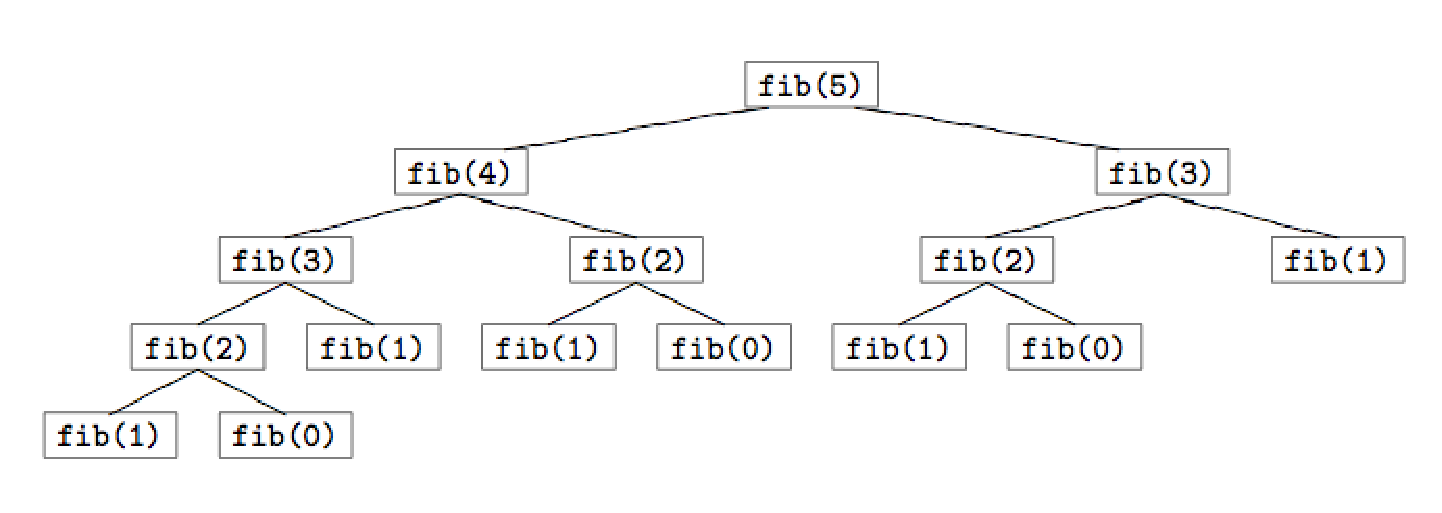
\epsfig{file=Abbildungen/fibonacci.eps, scale=0.6}} 
  \caption{Rekursions-Baum f\"{u}r die Berechnung von $\textsl{fibonacci}(5)$.}
  \label{fig:fibonacci.eps}
\end{figure}


Wir k\"{o}nnen eine effizientere Berechnung der Fibonacci-Zahlen implementieren, indem wir
uns die berechneten Werte merken.  Dazu k\"{o}nnen wir eine Liste benutzen.
 Dies f\"{u}hrt zu dem in Abbildung \ref{fig:fibonacci-dynamic}
auf Seite \pageref{fig:fibonacci-dynamic} angegebenen Programm.  
 Da die Fibonacci-Zahlen $f_n$ mit $n=0$ beginnen, die Elemente einer Liste aber mit
1 beginnend indiziert werden, wird der Wert
\\[0.2cm]
\hspace*{1.3cm}
$\textsl{fibonacci(i)}$ \quad in der Liste $l$ an der Stelle \quad $l(i+1)$
\\[0.2cm]
gespeichert. 

\begin{figure}[!h]
  \centering
\begin{Verbatim}[ frame         = lines, 
                  framesep      = 0.3cm, 
                  labelposition = bottomline,
                  numbers       = left,
                  numbersep     = -0.2cm,
                  xleftmargin   = 0.8cm,
                  xrightmargin  = 0.8cm
                ]
    fibonacci := procedure(n) {
        l := [1, 1] + [2 .. n];
        for (k in [ 2 .. n ]) {
            l(k+1) := l(k) + l(k-1);
        }
        return l(n+1);
    };
    
    for (n in [0 .. 10000]) {
        print("fibonacci($n$) = $fibonacci(n)$");
    }
\end{Verbatim}
\vspace*{-0.3cm}
  \caption{Berechnung der Fibonacci-Zahlen mit Speicherung der Zwischenwerte.}
  \label{fig:fibonacci-dynamic}
\end{figure} 


\section{Lineare Rekurrenz-Gleichung \label{sec:lineare-RG}}
Wir waren bei der Analyse der Komplexit\"{a}t des ersten Programms zur Berechnung der
Fibonacci-Zahlen auf die Gleichung \\[0.2cm]
\hspace*{1.3cm} $a_{i+2} = a_{i+1} + {a_i} + 1$ \quad f\"{u}r alle $i \in \mathbb{N}$ \\[0.2cm]
gesto\3en. Gleichungen dieser Form treten bei der Analyse der Komplexit\"{a}t rekursiver
Programme h\"{a}ufig auf. Wir wollen uns daher in diesem Abschnitt n\"{a}her mit solchen
Gleichungen besch\"{a}ftigen.

\begin{Definition}[Lineare homogene Rekurrenz-Gleichung] \hspace*{\fill} \\
{\em 
  Die \emph{lineare homogene Rekurrenz-Gleichung der Ordnung $k$ mit konstanten Koeffizienten} hat die Form
  \begin{equation}
    \label{eq:lhrg}
  a_{n+k} = c_{k-1} \cdot a_{n+k-1} + c_{k-2} \cdot a_{n+k-2} + \cdots + c_1 \cdot a_{n+1} + c_0 \cdot a_{n}
     \quad \mbox{f\"{u}r alle $n \in \mathbb{N}$}. 
  \end{equation}
     In Summen-Schreibweise kann diese Gleichung kompakter als 
     \\[0.2cm]
     \hspace*{1.3cm}
     $a_{n+k} = \sum\limits_{i=0}^{k-1} c_i \cdot a_{n+i}$ \quad f\"{u}r alle $n \in \mathbb{N}$
     \\[0.2cm]
     geschreiben werden.
     Zus\"{a}tzlich werden \emph{Anfangs-Bedingungen}  
      \\[0.2cm]
      \hspace*{1.3cm}      
      $a_0 = d_0, \cdots, a_{k-1} = d_{k-1}$ 
      \\[0.2cm]
      f\"{u}r die Folge $\folge{a_n}$ vorgegeben.    
    \hspace*{\fill} $\Box$
}
\end{Definition}
Durch eine lineare homogene Rekurrenz-Gleichung wird die Folge $(a_n)_{n\in\mathbb{N}}$
eindeutig bestimmt: Die Werte $a_n$ f\"{u}r $n < k$ sind durch die Anfangs-Bedingungen gegeben und
alle weiteren Werte k\"{o}nnen dann durch die Rekurrenz-Gleichung (\ref{eq:lhrg}) bestimmt werden.
Noch  etwas zur Nomenklatur:
\begin{enumerate}
\item Die Rekurrenz-Gleichung (\ref{eq:lhrg}) hei\3t \emph{linear}, weil die Glieder der Folge $(a_n)_n$ nur
      linear in der Gleichung (\ref{eq:lhrg}) auftreten.  Ein Beispiel f\"{u}r eine
      Rekurrenz-Gleichung, die nicht linear ist, w\"{a}re \\[0.2cm]
      \hspace*{1.3cm} $a_{n+1} = a_n^2$ \quad f\"{u}r alle $n \in \mathbb{N}$. \\[0.2cm]
      Nicht-lineare Rekurrenz-Gleichungen sind nur in Spezialf\"{a}llen geschlossen l\"{o}sbar.
\item Die Rekurrenz-Gleichung (\ref{eq:lhrg}) hei\3t \emph{homogen}, weil auf der rechten Seite
      dieser Gleichung kein konstantes Glied mehr auftritt.  Ein Beispiel f\"{u}r eine
      Gleichung, die nicht homogen ist (wir sprechen auch von \emph{inhomogenen}
      Rekurrenz-Gleichungen), w\"{a}re \\[0.2cm]
      \hspace*{1.3cm} $a_{n+2} = a_{n+1} + a_n + 1$ \quad f\"{u}r alle $n \in \mathbb{N}$. \\[0.2cm]
      Mit inhomogenen Rekurrenz-Gleichungen werden wir uns sp\"{a}ter noch besch\"{a}ftigen.
\item Die Rekurrenz-Gleichung (\ref{eq:lhrg}) hat \emph{konstante Koeffizienten}, weil die
      Werte $c_i$ Konstanten sind, die nicht von dem Index $n$ abh\"{a}ngen.  Ein Beispiel f\"{u}r
      eine Rekurrenz-Gleichung, die keine konstanten Koeffizienten hat, ist \\[0.2cm]
      \hspace*{1.3cm} $a_{n+1} = n\cdot a_n$ \quad f\"{u}r alle $n \in \mathbb{N}$. \\[0.2cm]
      Solche Rekurrenz-Gleichungen k\"{o}nnen in vielen F\"{a}llen auf Rekurrenz-Gleichungen mit
      konstanten Koeffizienten zur\"{u}ck gef\"{u}hrt werden.  Wir werden das sp\"{a}ter noch im
      Detail besprechen.
\end{enumerate}
Wie l\"{o}sen wir eine lineare homogene Rekurrenz-Gleichung?  Wir versuchen zun\"{a}chst den Ansatz\\[0.2cm]
\hspace*{1.3cm}  $a_n = \lambda^n$ \quad f\"{u}r alle $n \in \mathbb{N}$. \\[0.2cm]
Einsetzen dieses Ansatzes in (\ref{eq:lhrg}) f\"{u}hrt auf die Gleichung \\[0.2cm]
\hspace*{1.3cm}
$\lambda^{n+k} = \sum\limits_{i=0}^{k-1} c_i \cdot \lambda^{n+i}$
\\[0.2cm]
Dividieren wir diese Gleichung durch $\lambda^n$, so haben wir: \\[0.2cm]
\hspace*{1.3cm} $\lambda^{k} = \sum\limits_{i=0}^{k-1} c_i \cdot \lambda^{i}$  
\\[0.2cm]
Das Polynom \\[0.2cm]
\hspace*{1.3cm} 
$\chi(x) = x^{k} - \sum\limits_{i=0}^{k-1} c_i \cdot x^{i}$  
\\[0.2cm]
 hei\3t \emph{charakteristisches Polynom} der Rekurrenz-Gleichung (\ref{eq:lhrg}).
Wir betrachten zun\"{a}chst den Fall, dass das charakteristische  Polynom  $k$  verschiedene
Nullstellen hat.  In diesem Fall sagen, dass die Rekurrenz-Gleichung (\ref{eq:lhrg}) 
\emph{nicht entartet} ist.
Bezeichnen wir diese Nullstellen mit \\[0.2cm]
\hspace*{1.3cm}  $\lambda_1$, $\lambda_2$, $\cdots$, $\lambda_k$, \\[0.2cm]
so  gilt f\"{u}r alle $j = 1,\cdots, k$ \\[0.2cm]
\hspace*{1.3cm} 
$\lambda_j^{n+k} = \sum\limits_{i=0}^{k-1} c_i \cdot \lambda_j^{n+i}$.
\\[0.2cm]
Damit ist die Folge  
\[\bigl(\lambda_j^n)_{n\in\mathbb{N}}\]
f\"{u}r alle $j=1,\cdots,k$ eine L\"{o}sung der Rekurrenz-Gleichung (\ref{eq:lhrg}).
Au\3erdem ist auch jede Linear-Kombination dieser L\"{o}sungen eine L\"{o}sung von (\ref{eq:lhrg}):
Definieren wir die Folge $a_n$ durch \\[0.2cm]
\hspace*{1.3cm} 
$a_n = \alpha_1 \cdot \lambda_1^n + \cdots + \alpha_k \cdot \lambda_k^n$ \quad f\"{u}r alle $n
\in \mathbb{N}$ 
\\[0.2cm]
mit beliebigen Koeffizienten $\alpha_i \in \mathbb{R}$, so erf\"{u}llt auch die Folge
$(a_n)_n$ die Gleichung (\ref{eq:lhrg}).  Die oben definierte Folge $(a_n)_n$ bezeichnen wir als
die  \emph{allgemeine L\"{o}sung} der Rekurrenz-Gleichung (\ref{eq:lhrg}). 
Die Koeffizienten $\alpha_i$ m\"{u}ssen wir f\"{u}r $i=1,\;\cdots,\;k$ so w\"{a}hlen, dass die
Anfangs-Bedingungen 
\\[0.2cm]
\hspace*{1.3cm}
$a_0 = d_0$, $\cdots$, $a_{k-1} = d_{k-1}$
\\[0.2cm]
erf\"{u}llt sind.  Das liefert ein lineares Gleichungs-System f\"{u}r die Koeffizienten $\alpha_1$, $\cdots$, $\alpha_k$:
\[
\begin{array}{lcl}
  d_0     & = & \lambda_1^0 \cdot \alpha_1 + \cdots +   \lambda_k^0 \cdot \alpha_k \\[0.2cm]
  d_1     & = & \lambda_1^1 \cdot \alpha_1 + \cdots +   \lambda_k^1 \cdot \alpha_k \\[0.2cm]
  \vdots  &   & \vdots                                                   \\[0.2cm]
  d_{k-1} & = & \lambda_1^{k-1} \cdot \alpha_1 + \cdots +   \lambda_{k}^{k-1} \cdot \alpha_k \\[0.2cm]
\end{array}
\]
Hier sind die Werte $\lambda_i$  die Nullstellen des charakteristischen Polynoms.  
Die Matrix $V$, die diesem Gleichungs-System
zugeordnet ist, lautet: 
\[
V = \left(
\begin{array}{lcl}
  \lambda_1^0  & \cdots &   \lambda_k^0 \\[0.2cm]
  \lambda_1^1  & \cdots &   \lambda_k^1 \\[0.2cm]
  \vdots         &         & \vdots \\[0.2cm]
  \lambda_1^{k-1} & \cdots &   \lambda_{k}^{k-1} \\[0.2cm]
\end{array}\right)
\]
Diese Matrix ist in der Mathematik als \emph{Vandermonde}'sche Matrix bekannt.  
Es l\"{a}sst sich zeigen, dass ein Gleichungs-System, das mit dieser Matrix gebildet wird,
genau dann eindeutig l\"{o}sbar ist, wenn die Nullstellen $\lambda_i$ f\"{u}r $i=1,\cdots,k$
paarweise verschieden sind.
\vspace*{0.2cm}

\noindent
\textbf{Beispiel}:  Wie demonstrieren das Verfahren an einem Beispiel: Wie betrachten die
Rekurrenz-Gleichung \\[0.2cm]
\hspace*{1.3cm} $F_{n+2} = F_{n+1} + F_{n}$ \quad f\"{u}r alle $n \in \mathbb{N}$  \\[0.2cm]
mit den Anfangs-Bedingungen $F_0 = 0$ und $F_1 = 1$.  Die L\"{o}sung dieser
Rekurrenz-Gleichung sind \"{u}brigens gerade die Fibonacci-Zahlen.
Das \emph{charakteristische Polynom} dieser Rekurrenz-Gleichung lautet: \\[0.2cm]
\hspace*{1.3cm} $\chi(x) = x^2 - x - 1$.  \\[0.2cm]
Das f\"{u}hrt auf die quadratische Gleichung \\[0.2cm]
\hspace*{1.3cm} $x^2 -x - 1 = 0$ \\[0.2cm]
Wir haben eben schon gesehen, dass diese quadratische Gleichung die L\"{o}sung \\[0.2cm]
\hspace*{1.3cm}
 $ x_{1/2} = \frac{1}{2} \cdot (1 \pm \sqrt{5})$ 
\\[0.2cm]
hat.  Wir definieren \\[0.2cm]
\hspace*{1.3cm} 
$\lambda_1 = \frac{1}{2} \cdot (1 + \sqrt{5})$ \quad und  \quad 
$\lambda_2 = \frac{1}{2} \cdot (1 - \sqrt{5})$. \\[0.2cm]
Damit lautet die \emph{allgemeine L\"{o}sung} der betrachteten Rekurrenz-Gleichung \\[0.2cm]
\hspace*{1.3cm}  $F_n = \alpha_1 \cdot \lambda_1^n  + \alpha_2 \cdot \lambda_2^n$ \quad f\"{u}r alle $n \in \mathbb{N}$. \\[0.2cm]
Setzen wir hier die Anfangs-Bedingungen ein, so erhalten wir
\[
\begin{array}{lcl}
    0 & = & \lambda_1^0 \cdot \alpha_1 + \lambda_2^0   \cdot \alpha_2 \\[0.2cm]
    1 & = & \lambda_1^1 \cdot \alpha_1 + \lambda_2^{1} \cdot \alpha_2 
\end{array}
\]
Dies ist ein lineares Gleichungs-System in den Unbekannten $\alpha_1$ und
$\alpha_2$. Vereinfachung f\"{u}hrt auf 
\[
\begin{array}{lcl}
    0 & = & \alpha_1 + \alpha_2 \\[0.2cm]
    1 & = & \lambda_1 \cdot \alpha_1 + \lambda_2 \cdot \alpha_2 
\end{array}
\]
Die erste dieser beiden Gleichungen l\"{o}sen wir nach $\alpha_2$ auf und finden  $\alpha_2 = - \alpha_1$.
Diesen Wert setzen wir in der zweiten Gleichung ein.  Das f\"{u}hrt auf
\[
\begin{array}{lrcl}
                 & 1 & = & \lambda_1 \cdot \alpha_1 - \lambda_2 \cdot \alpha_1 \\[0.2cm]
 \Leftrightarrow & 1 & = & (\lambda_1 - \lambda_2) \cdot \alpha_1              \\[0.2cm]
 \Leftrightarrow & \bruch{1}{\lambda_1 - \lambda_2} & = & \alpha_1 
\end{array}
\]
Setzen wir diesen Wert in die Gleichung $\alpha_2 = - \alpha_1$ ein, so erhalten wir \\[0.2cm]
\hspace*{1.3cm} 
  $\alpha_2 = \bruch{- 1}{\lambda_1 - \lambda_2}$.
\\[0.2cm]
Setzen wir die  Werte f\"{u}r $\lambda_1$ und $\lambda_2$ ein, so finden wir:  \\[0.2cm]
\hspace*{1.3cm} 
$\alpha_1 = \bruch{1}{\sqrt{5}}$ \quad und \quad $\alpha_2 = - \bruch{1}{\sqrt{5}}$.
\\[0.2cm]
Die L\"{o}sung der Rekurrenz-Gleichung \\[0.2cm]
\hspace*{1.3cm} $F_{n+2} = F_{n+1} + F_{n}$ \quad f\"{u}r alle $n \in \mathbb{N}$ \\[0.2cm]
mit den Anfangs-Bedingungen $F_0 = 1$ und $F_1 = 1$   lautet also 
\\[0.2cm]
\hspace*{1.3cm} 
$F_n = \bruch{1}{\sqrt{5}}\cdot \left( \lambda_1^{n} - \lambda_2^{n} \right)$ 
\quad f\"{u}r alle $n \in \mathbb{N}$.  
\\[0.2cm]
Damit haben wir eine geschlossene Formel zur Berechnung der Fibonacci-Zahlen
gefunden.  Diese Formel zeigt uns, dass die Fibonacci-Zahlen selbst exponentiell anwachsen.
Wir werden diese Formel sp\"{a}ter bei der Analyse des Laufzeitverhaltens des
Euklidischen-Algorithmus ben\"{o}tigen. 

\vspace*{0.2cm}
\noindent
\textbf{Aufgabe}:  L\"{o}sen Sie die Rekurrenz-Gleichung 
$a_{n+2} = \bruch{3}{2} \cdot a_{n+1} - \bruch{1}{2}\cdot a_n$ mit
den Anfangs-Bedingungen $a_0 = 3$ und $a_1 = \bruch{5}{2}$.

%\noindent
%\textbf{L\"{o}sung}: $a_n = 2 + \left(\frac{1}{2}\right)^n$.

\subsection{Entartete Rekurrenz-Gleichungen}
Wir hatten oben zun\"{a}chst den Fall betrachtet, dass das charakteristische Polynom der
Rekurrenz-Gleichung (\ref{eq:lhrg}) insgesamt $k$ verschiedene Nullstellen hat.   Dies muss
keineswegs immer der Fall sein.  Wir betrachten die Rekurrenz-Gleichung 
\begin{equation}
  \label{eq:erg}
  a_{n+2} = 4 \cdot a_{n+1} - 4 \cdot a_n \quad \mbox{f\"{u}r alle $n \in \mathbb{N}$} 
\end{equation}
 mit den Anfangs-Bedingungen $a_0 = 1$, $a_1 = 4$.  Das charakteristische Polynom lautet \\[0.2cm]
\hspace*{1.3cm} $\chi(x) = x^2 - 4 \cdot x + 4 = (x - 2)^2$ \\[0.2cm]
und hat offensichtlich nur eine Nullstelle bei $x = 2$.   Eine L\"{o}sung der
Rekurrenz-Gleichung (\ref{eq:erg}) lautet daher \\[0.2cm]
\hspace*{1.3cm} $a_n = 2^n$ \quad f\"{u}r alle $n \in \mathbb{N}$. \\[0.2cm]
Eine weitere L\"{o}sung ist \\[0.2cm]
\hspace*{1.3cm} $a_n = n \cdot 2^n$ \quad f\"{u}r alle $n \in \mathbb{N}$.  \\[0.2cm]
Wir verifizieren dies durch Einsetzen: 
\[
\begin{array}{llcll}
 & (n+2) \cdot 2^{n+2} & = & 4 \cdot (n+1) \cdot 2^{n+1} - 4 \cdot n \cdot 2^n & \mid\; \div 2^n \\
\Leftrightarrow & 
   (n+2) \cdot 2^{2} & = & 4 \cdot (n+1) \cdot 2^{1} - 4 \cdot n  &  \mid\; \div 4 \\
\Leftrightarrow & n + 2 & = & (n + 1) \cdot 2 -  n  &  \\
\Leftrightarrow & n + 2 & = & 2 \cdot n + 2 -  n   \\
\Leftrightarrow & n + 2 & = & n + 2    \\
\end{array}
\]
Die allgemeine L\"{o}sung der Rekurrenz-Gleichung finden wir durch Linear-Kombination der
beiden L\"{o}sungen: \\[0.2cm]
\hspace*{1.3cm} $a_n = \alpha \cdot 2^n + \beta \cdot n \cdot 2^n$ \quad f\"{u}r alle $n \in \mathbb{N}$. \\[0.2cm]
Setzen wir hier die Anfangs-Bedingungen $a_0 = 1$ und $a_2 = 4$ ein, so erhalten wir:
\[
\left\{
\begin{array}{lcl}
  1 & = & \alpha \cdot 2^0 + \beta \cdot 0 \cdot 2^0 \\
  4 & = & \alpha \cdot 2^1 + \beta \cdot 1 \cdot 2^1 \\
\end{array}
\right\} \quad\Leftrightarrow\quad \left\{
\begin{array}{lcl}
  1 & = & \alpha \\
  4 & = & \alpha \cdot 2 + \beta \cdot 2 \\
\end{array}
\right\}\]
Die L\"{o}sung lautet offenbar $\alpha = 1$ und $\beta = 1$.  Damit lautet die L\"{o}sung der
Rekurrenz-Gleichung (\ref{eq:erg}) mit den Anfangs-Bedingungen $a_0 = 1$ und $a_2 = 4$ \\[0.2cm]
\hspace*{1.3cm} $a_n = 2^n + n \cdot 2^n = (n+1) \cdot 2^n$ \quad f\"{u}r alle $n \in \mathbb{N}$.  \\[0.2cm]
Im allgemeinen nennen wir die Rekurrenz-Gleichung \\[0.2cm]
\hspace*{1.3cm} $a_{n+k} = \sum\limits_{i=0}^{k-1} c_{i} \cdot a_{n+i}$ \\[0.2cm]
\emph{entartet}, wenn das charakteristische Polynom \\[0.2cm]
\hspace*{1.3cm} $\chi(x) = x^k - \sum\limits_{i=0}^{k-1} c_{i} \cdot x^{i}$  \\[0.2cm]
weniger als $k$ verschiedene Nullstellen hat.  Dann l\"{a}sst sich folgendes
zeigen:  Hat das charakteristische Polynom $\chi(x)$ eine $r$-fache Nullstelle
$\lambda$, gilt also \\[0.2cm]
\hspace*{1.3cm} $\chi(x) = (x - \lambda)^r \cdot \phi(x)$ \\[0.2cm]
mit einem geeigneten Polynom $\phi(x)$, so sind die Folgen
\begin{enumerate}
\item $(\lambda^n)_{n\in\mathbb{N}}$
\item $(n\cdot\lambda^n)_{n\in\mathbb{N}}$
\item $(n^2\cdot\lambda^n)_{n\in\mathbb{N}}$
\item $\vdots$
\item $(n^{r-1}\cdot\lambda^n)_{n\in\mathbb{N}}$
\end{enumerate}
L\"{o}sungen der Rekurrenz-Gleichung (\ref{eq:erg}).  Durch eine geeignete Linear-Kombination dieser
L\"{o}sungen zusammen mit den L\"{o}sungen, die sich aus den anderen Nullstellen des Polynoms $\phi$
ergeben, l\"{a}sst sich dann immer eine L\"{o}sung finden, die auch den Anfangs-Bedingungen gen\"{u}gt.
\vspace*{0.3cm}

\noindent
\textbf{Aufgabe}: L\"{o}sen Sie die Rekurrenz-Gleichung \\[0.2cm]
\hspace*{1.3cm} $a_{n+3} = a_{n+2} + a_{n+1} - a_n$ \\[0.2cm]
f\"{u}r die Anfangs-Bedingungen $a_0 = 0$, $a_1 = 3$, $a_2 = 2$.

%\noindent
%\textbf{L\"{o}sung}: allg. $a_n = \alpha + n \cdot \beta + \gamma \cdot (-1)^n$. 
%Anfangs-Bedingungen: $a_n = 1 + n - (-1)^n$.
\pagebreak

\subsection{Inhomogene Rekurrenz-Gleichungen}    
\begin{Definition}[Lineare inhomogene Rekurrenz-Gleichung] \lb
{\em Die \emph{lineare \underline{inhomo}g\underline{ene} Rekur\-renz-Gleichung der Ordnung
$k$ mit konstanten Koeffizienten und konstanter Inhomogenit\"{a}t} hat die Form 
\begin{equation}
  \label{eq:lihrg}
     a_{n+k} = \sum\limits_{i=0}^{k-1} c_{i} \cdot a_{n+i} + c_{-1}  
\end{equation}
     mit den Anfangs-Bedingungen $a_0 = d_0$, $\cdots$, $a_{k-1} = d_{k-1}$. 
     Dabei gilt f\"{u}r die Koeffizienten \\[0.2cm]
     \hspace*{1.3cm} $c_i \in \mathbb{R}$ \quad f\"{u}r alle $i = -1, 0,\cdots, k-1$. \\[0.2cm]
     F\"{u}r die  \emph{Anfangs-Bedingungen} $d_0, \cdots, d_{k-1}$ gilt ebenfalls \\[0.2cm]
     \hspace*{1.3cm} $d_i \in \mathbb{R}$ \quad f\"{u}r alle $i = 0,\cdots, k-1$. \\[0.2cm]
     Die Konstante $c_{-1}$ bezeichnen wir als die \emph{Inhomogenit\"{a}t}. 
     \hspace*{\fill} $\Box$
}
\end{Definition}

Wie l\"{a}sst sich die inhomogene Rekurrenz-Gleichung (\ref{eq:lihrg}) l\"{o}sen? Wir zeigen
zun\"{a}chst, wie sich eine \emph{spezielle L\"{o}sung} der Rekurrenz-Gleichung (\ref{eq:lihrg})
finden l\"{a}sst.  Dazu betrachten wir das charakteristische Polynom \\[0.2cm]
\hspace*{1.3cm} 
$\chi(x) = x^k - \sum\limits_{i=0}^{k-1} c_{i} \cdot x^i$
\\[0.2cm]
und definieren die \emph{Spur} $\mathtt{sp}(\chi)$ wie folgt: \\[0.2cm]
\hspace*{1.3cm} 
$\mathtt{sp}(\chi) := \chi(1) = 1 - \sum\limits_{i=0}^{k-1} c_{i}$. \\[0.2cm]
Es k\"{o}nnen zwei F\"{a}lle auftreten, $\mathtt{sp}(\chi) \not= 0$ und
$\mathtt{sp}(\chi) = 0$.
Wir betrachten die beiden F\"{a}lle getrennt.
\begin{enumerate}
\item $\mathtt{sp}(\chi) \not= 0$.

      Dann erhalten wir eine spezielle L\"{o}sung von (\ref{eq:lihrg}) durch den Ansatz \\[0.2cm]
      \hspace*{1.3cm} $a_n = \delta$ \quad f\"{u}r alle $n \in \mathbb{N}$. \\[0.2cm]
      Den Wert von $\delta$ bestimmen wir durch Einsetzen, es muss f\"{u}r alle $n\in \mathbb{N}$ gelten: \\[0.2cm]
      \hspace*{1.3cm} 
      $\delta = \sum\limits_{i=0}^{k-1} c_{i} \cdot \delta + c_{-1}$.
      \\[0.2cm]
      Daraus ergibt sich \\[0.2cm]
      \hspace*{1.3cm} 
      $\delta \cdot \left(1 - \sum\limits_{i=0}^{k-1} c_{i} \right) =  c_{-1}$. \\[0.2cm]
      Das ist aber nichts anderes als \\[0.2cm]
      \hspace*{1.3cm} $\delta \cdot \mathtt{sp}(\chi) = c_{-1}$ \\[0.2cm]
      und damit lautet eine spezielle L\"{o}sung von (\ref{eq:lihrg}) \\[0.2cm]
      \hspace*{1.3cm} $a_n = \delta = \bruch{c_{-1}}{\mathtt{sp}(\chi)}$.
      \\[0.2cm]
      Jetzt sehen wir auch, warum die Voraussetzung $\mathtt{sp}(\chi) \not= 0$
      wichtig ist, denn anderfalls w\"{a}re der Quotient
      $\bruch{c_{-1}}{\mathtt{sp}(\chi)}$ undefiniert.
\item $\mathtt{sp}(\chi) = 0$.

      In diesem Fall versuchen wir, eine spezielle L\"{o}sung von (\ref{eq:lihrg}) durch den
      Ansatz \\[0.2cm]
      \hspace*{1.3cm} $a_n = \varepsilon \cdot n $ \\[0.2cm]
      zu finden.  Den Wert $\varepsilon$ erhalten wir durch Einsetzen, es muss f\"{u}r 
      alle $n\in\mathbb{N}$ gelten: \\[0.2cm]
      \hspace*{1.3cm} 
      $\varepsilon \cdot (n + k) = \sum\limits_{i=0}^{k-1} c_{i} \cdot \varepsilon \cdot (n + i) + c_{-1}$  
      \\[0.2cm]
      Dies formen wir wie folgt um:
      \[
        \varepsilon \cdot n + \varepsilon \cdot k = 
        \varepsilon \cdot n \cdot \sum\limits_{i=0}^{k-1} c_{i} +
        \varepsilon \cdot \sum\limits_{i=0}^{k-1} i \cdot c_{i} + c_{-1} 
      \]
      Aus  $\mathtt{sp}(\chi) = 0$ folgt $1  =  \sum\limits_{i=0}^{k-1} c_i$
      und damit gilt \\[0.2cm]
      \hspace*{1.3cm} 
      $\varepsilon \cdot n = \varepsilon \cdot n \cdot \sum\limits_{i=0}^{k-1} c_{i}$.
      \\[0.2cm]
      Daher vereinfacht sich die obige Gleichung zu 
      \[
      \begin{array}{ll}
      & \varepsilon \cdot k = \varepsilon \cdot \sum\limits_{i=0}^{k-1} i \cdot c_{i} + c_{-1} \\[0.4cm]
      \Leftrightarrow\quad 
      & \varepsilon \cdot \left(k - \sum\limits_{i=0}^{k-1} i \cdot c_{i}\right) = c_{-1} 
      \\[0.5cm]
      \Leftrightarrow\quad 
      & \varepsilon = \frac{\displaystyle c_{-1}}{\displaystyle \; k - \sum\limits_{i=0}^{k-1} i \cdot c_{i}\;} 
      \end{array}
      \]
      Wenn wir genau hin schauen, dann sehen wir, dass der Wert im Nenner nicht anderes ist
      als der Wert der Ableitung des charakteristischen Polynoms an der Stelle 1, denn es gilt: \\[0.2cm]
      \hspace*{1.3cm} 
      $\chi'(x) =\frac{d\;}{dx}\chi(x) = k \cdot x^{k-1} - \sum\limits_{i=1}^{k-1} c_{i}\cdot i \cdot x^{i-1}$
      \\[0.2cm]
      Setzen wir hier f\"{u}r $x$ den Wert $1$ ein, so finden wir \\[0.2cm]
      \hspace*{1.3cm} 
      $\chi'(1) = k - \sum\limits_{i=1}^{k-1} c_{i}\cdot i =  k - \sum\limits_{i=0}^{k-1} c_{i}\cdot i$. 
      \\[0.2cm]
      Insgesamt haben wir damit also die folgende spezielle L\"{o}sung $(a_n)_{n\in\mathbb{N}}$
      der Gleichung (\ref{eq:lihrg}) gefunden: \\[0.2cm]
      \hspace*{1.3cm} $a_n = \bruch{c_{-1}}{\;\chi'(1)\;}\cdot n$.

      Wir haben oben zur Vereinfachung angenommen, dass dieser Wert von 0 verschieden ist,
      dass also das charakteristische Polynom $\chi(x)$ an der Stelle $x=1$ keine mehrfache
      Nullstelle hat, denn nur dann ist $\varepsilon$ durch die
      obige Gleichung wohldefiniert und wir haben eine spezielle L\"{o}sung der
      Rekurrenz-Gleichung (\ref{eq:lihrg}) gefunden.  Andernfalls k\"{o}nnen wir die Reihe nach die
      Ans\"{a}tze $a_n = \varepsilon \cdot n^2$, $a_n = \varepsilon \cdot n^3$ , $\cdots$
      versuchen, denn es kann folgendes gezeigt werden: 
      Hat das charakteristische Polynom $\chi(x)$ am Punkt $x = 1$ eine Nullstelle vom Rang $r$,
      so f\"{u}hrt der Ansatz $a_n = \varepsilon \cdot n^r$ zu einer speziellen L\"{o}sung von (\ref{eq:lihrg}).
\end{enumerate}
Diese spezielle L\"{o}sung gen\"{u}gt i.~a.~noch nicht den
Anfangs-Bedingungen. Eine L\"{o}sung, die auch den Anfangs-Bedingungen gen\"{u}gt, erhalten wir,
wenn wir zu der speziellen L\"{o}sung die allgemeine L\"{o}sung der zugeh\"{o}rigen homogenen linearen
Rekurrenz-Gleichung \\[0.2cm]
\hspace*{1.3cm} 
     $a_{n+k} = c_{k-1} \cdot a_{n+k-1} + c_{k-2} \cdot a_{n+k-2} + \cdots + c_1 \cdot a_{n+1} + c_0 \cdot a_{n}$ 
\\[0.2cm]
addieren und die Koeffizienten der allgemeinen L\"{o}sung so w\"{a}hlen, dass die
Anfangs-Bedingungen erf\"{u}llt sind.  Wir betrachten  ein Beispiel:
 Die zu l\"{o}sende Rekurrenz-Gleichung lautet \\[0.2cm]
\hspace*{1.3cm} $a_{n+2} = 3 \cdot a_{n+1} - 2 \cdot a_n -1$ \quad f\"{u}r alle $n \in \mathbb{N}$. \\[0.2cm]
Die Anfangs-Bedingungen sind $a_0 = 1$ und $a_1 = 3$.  Wir berechnen zun\"{a}chst eine
spezielle L\"{o}sung.  Das charakteristische Polynom ist \\[0.2cm]
\hspace*{1.3cm} $\chi(x) = x^2 -3 \cdot x +2 = (x - 1) \cdot (x - 2)$. \\[0.2cm]
Es gilt $\mathtt{sp}(\chi) = \chi(1) = 0$.  Wir versuchen f\"{u}r die spezielle L\"{o}sung
den Ansatz \\[0.2cm]
\hspace*{1.3cm} $a_n = \varepsilon \cdot n$. \\[0.2cm]
Einsetzen in die Rekurrenz-Gleichung liefert \\[0.2cm]
\hspace*{1.3cm}  $\varepsilon \cdot (n+2) = 3 \cdot \varepsilon \cdot(n+1) - 2 \cdot \varepsilon \cdot n -1$ \quad f\"{u}r alle $n \in \mathbb{N}$. \\[0.2cm]
Das ist \"{a}quivalent zu \\[0.2cm]
\hspace*{1.3cm} $\varepsilon \cdot (2 - 3) = - 1$ \\[0.2cm]
und daraus folgt sofort $\varepsilon = 1$.  Damit lautet eine spezielle L\"{o}sung \\[0.2cm]
\hspace*{1.3cm} $a_n = n$ \quad f\"{u}r alle $n \in \mathbb{N}$. \\[0.2cm]
Da die Nullstellen des charakteristischen Polynoms $\chi(x)$ bei 1 und 2 liegen, finden
wir f\"{u}r die allgemeine L\"{o}sung 
\\[0.2cm]
\hspace*{1.3cm} $a_n = \alpha \cdot 1^n + \beta \cdot 2^n + n$ \quad f\"{u}r alle $n \in \mathbb{N}$. \\[0.2cm]
Setzen wir hier f\"{u}r $n$ die Werte $0$ und $1$ und f\"{u}r $a_n$ die beiden Anfangs-Bedingungen
ein, so erhalten wir das Gleichungs-System \\[0.2cm]
\[ \left\{
\begin{array}{lcl}
1 &=& \alpha \cdot 1^0 + \beta \cdot 2^0 + 0 \\
3 &=& \alpha \cdot 1^1 + \beta \cdot 2^1 + 1
\end{array} \right\} \Leftrightarrow \left\{
\begin{array}{lcl}
1 &=& \alpha + \beta  \\
3 &=& \alpha + 2 \cdot \beta + 1
\end{array} \right\}\]
Sie k\"{o}nnen leicht nachrechnen, dass dieses Gleichungs-System die L\"{o}sung $\alpha = 0$ und
$\beta = 1$ hat.  Damit lautet die L\"{o}sung der Rekurrenz-Gleichung \\[0.2cm]
\hspace*{1.3cm} $a_n = 2^n + n$ \quad f\"{u}r alle $n \in \mathbb{N}$.
\vspace*{0.3cm}

\noindent
\textbf{Aufgabe}: L\"{o}sen Sie die inhomogene Rekurrenz-Gleichung \\[0.2cm]
\hspace*{1.3cm} $a_{n+2} = 2 \cdot a_n - a_{n+1} + 3$ \\[0.2cm]
f\"{u}r die Anfangs-Bedingungen $a_0 = 2$ und $a_1 = 1$.
% charakteristisches Polynom: $\chi(x) = x^2 + x - 2 = (x - 1) * (x + 2)
% sp(\chi) = 0, \chi'(x) = 2*x + 1, \chi'(1) = 3
% Lsg: a_n = \varepsilon * n mit \varepsilon = 1
% Lsg: a_n = 4/3 + 2/3*(-2)^n + n

\subsection{Lineare inhomogene Rekurrenz-Gleichungen mit ver\"{a}nderlichen Inhomogenit\"{a}ten}
Gelegentlich tauchen in der Praxis Rekurrenz-Gleichungen auf, in denen die Inhomogenit\"{a}t
keine Konstante ist, sondern von $n$ abh\"{a}ngt.  In solchen F\"{a}llen f\"{u}hrt die
Technik des \emph{diskreten Differenzieren} oft zum Erfolg.  Wir stellen die Technik an
einem Beispiel vor und betrachten die Rekurrenz-Gleichung 
\begin{equation}
  \label{eq:dd}
a_{n+1} = 2 \cdot a_n + n \quad \mbox{f\"{u}r alle $n \in \mathbb{N}$}  
\end{equation}
und der Anfangs-Bedingungen $a_0 = 0$.  Das Verfahren zur L\"{o}sung solcher
Rekurrenz-Gleichung besteht aus vier Schritten:
\begin{enumerate}
\item Substitutions-Schritt: Im \emph{Substitutions-Schritt} setzen wir in der
      urspr\"{u}nglichen Rekurrenz-Gleichung (\ref{eq:dd}) f\"{u}r $n$ den Wert $n + 1$ ein und
      erhalten 
      \begin{equation}
        \label{eq:dd2}
        a_{n+2} = 2 \cdot a_{n+1} + n + 1 \quad \mbox{f\"{u}r alle $n \in \mathbb{N}$}
      \end{equation}
\item Subtraktions-Schritt: Im \emph{Subtraktions-Schritt} ziehen wir von der im
      Substitutions-Schritt erhaltenen Rekurrenz-Gleichung (\ref{eq:dd2}) die urspr\"{u}ngliche
      gegebene Rekurrenz-Gleichung (\ref{eq:dd}) ab.  In unserem Fall erhalten wir \\[0.2cm]
      \hspace*{1.3cm} 
      $a_{n+2} - a_{n+1} = 2 \cdot a_{n+1} + n + 1 - \left( 2 \cdot a_n + n \right)$ 
      \quad f\"{u}r alle $n \in \mathbb{N}$.       \\[0.2cm]
      Vereinfachung dieser Gleichung liefert 
      \begin{equation}
        \label{eq:dd3}
        a_{n+2} = 3 \cdot a_{n+1} - 2 \cdot a_n + 1 \quad \mbox{f\"{u}r alle $n \in \mathbb{N}$}.
      \end{equation}
      Die beiden Schritte 1.~und 2.~bezeichnen wir zusammen als 
      \emph{diskretes Differenzieren} der Rekurrenz-Gleichung.
\item Berechnung zus\"{a}tzlicher Anfangs-Bedingungen: Die Rekurrenz-Gleichung (\ref{eq:dd3})
      ist eine inhomogene Rekurrenz-Gleichung der Ordnung 2 mit nun aber konstanter
      Inhomogenit\"{a}t.  Wir haben bereits gesehen, 
      wie eine solche Rekurrenz-Gleichung zu l\"{o}sen ist, wir ben\"{o}tigen aber eine
      zus\"{a}tzliche Anfangs-Bedingung f\"{u}r $n=1$.  Diese erhalten wir, indem wir in der
      urspr\"{u}nglichen Rekurrenz-Gleichung (\ref{eq:dd}) f\"{u}r $n$ den Wert 0 einsetzen: \\[0.2cm]
      \hspace*{1.3cm} $a_1 = 2 \cdot a_0 + 0 = 0$.
\item L\"{o}sen der inhomogenen Rekurrenz-Gleichung mit konstanter Inhomogenit\"{a}t:
      Das charakteristische Polynom der Rekurrenz-Gleichung (\ref{eq:dd3}) lautet: \\[0.2cm]
      \hspace*{1.3cm} $\chi(x) = x^2 - 3 \cdot x + 2 = (x - 2) \cdot (x - 1)$. \\[0.2cm]
      Offenbar gilt $\mathtt{sp}(\chi) = 0$.  Um eine spezielle L\"{o}sung der
      Rekurrenz-Gleichung
      (\ref{eq:dd3}) zu erhalten, machen wir daher den Ansatz \\[0.2cm]
      \hspace*{1.3cm} $a_n = \varepsilon \cdot n$ \\[0.2cm]
      und erhalten \\[0.2cm]
      \hspace*{1.3cm} 
      $\varepsilon \cdot (n+2) = 3 \cdot \varepsilon \cdot (n+1) - 2 \cdot \varepsilon \cdot n + 1$ 
      \\[0.2cm]
      Diese Gleichung liefert die L\"{o}sung \\[0.2cm]
      \hspace*{1.3cm} 
      $\varepsilon = -1$. \\[0.2cm]
      Damit lautet die allgemeine L\"{o}sung der Rekurrenz-Gleichung (\ref{eq:dd3}): \\[0.2cm]
      \hspace*{1.3cm} $a_n = \alpha_1 \cdot 2^n + \alpha_2 \cdot 1^n - n$ \\[0.2cm]
      Die Koeffizienten $\alpha_1$ und $\alpha_2$ finden wir nun durch Einsetzen der
      Anfangs-Bedingungen:
      \[
      \begin{array}{lcl}
        0 & = & \alpha_1 + \alpha_2 \\
        0 & = & 2 \cdot \alpha_1 + \alpha_2 - 1 \\
      \end{array}
      \]
      Aus der ersten Gleichung folgt $\alpha_2 = - \alpha_1$.  Damit vereinfacht sich die
      zweite Gleichung zu \\[0.2cm]
      \hspace*{1.3cm} $0 = 2 \cdot \alpha_1 - \alpha_1 - 1$ \\[0.2cm]
      und damit lautet die L\"{o}sung $\alpha_1 = 1$ und $\alpha_2 = -1$.  Die L\"{o}sung der
      urspr\"{u}nglichen Rekurrenz-Gleichung (\ref{eq:dd}) mit der Anfangs-Bedingung $a_0 = 0$ 
      ist also \\[0.2cm]
      \hspace*{1.3cm} $a_n = 2^n - 1 - n$.
\end{enumerate}
Das oben gezeigte Verfahren funktioniert, wenn die Inhomogenit\"{a}t der Rekurrenz-Gleichung
linear ist, also die Form $\delta \cdot n$.  Ist die Inhomogenit\"{a}t quadratisch, so k\"{o}nnen wir
die Gleichung durch diskretes Differenzieren auf eine Rekurrenz-Gleichung reduzieren,
deren Inhomogenit\"{a}t linear ist.  Diese kann dann aber mit dem eben gezeigten Verfahren
gel\"{o}st werden.  Allgemein gilt:  Hat die Inhomogenit\"{a}t der Rekurrenz-Gleichung die Form \\[0.2cm]
\hspace*{1.3cm} $\delta \cdot n^r$ \quad $r \in \mathbb{N}$ und $r > 0$, \\[0.2cm]
so kann die Rekurrenz-Gleichung durch $r$-maliges diskretes Differenzieren auf eine
inhomogene Rekurrenz-Gleichung mit konstanter Inhomogenit\"{a}t reduziert werden.
\vspace*{0.3cm}
\pagebreak

\noindent
\textbf{Aufgabe}:  L\"{o}sen Sie die Rekurrenz-Gleichung \\[0.2cm]
\hspace*{1.3cm} $a_{n+1} = a_n + 2 \cdot n$ \quad f\"{u}r alle $n \in \mathbb{N}$ \\[0.2cm]
mit der Anfangs-Bedingung $a_0 = 0$.
\vspace*{0.3cm}

%\noindent
%\textbf{L\"{o}sung}: 
%\begin{enumerate}
%\item Charakteristisches Polynom: $\chi(x) = (x-1)^2$, doppelte Nullstelle! 
%\item Spezielle L\"{o}sung: $a_n = n^2$.
%\item Allgemeine L\"{o}sung: $a_n = \alpha_1 \cdot 1^n + \alpha_2 \cdot n \cdot 1^n + n^2$
%\item L\"{o}sung: $a_n = n\cdot(n-1)$.
%\end{enumerate}

\noindent
Die oben vorgestellte Technik des diskreten Differenzierens f\"{u}hrt in leicht variierter
Form oft auch dann noch zu einer L\"{o}sung, wenn die Inhomogenit\"{a}t nicht die Form eines
Polynoms hat.  Wir betrachten als Beispiel die Rekurrenz-Gleichung 
\begin{equation}
  \label{eq:expdd}
  a_{n+1} = a_n + 2^n \quad \mbox{f\"{u}r alle $n \in \mathbb{N}$}
\end{equation}
mit der Anfangs-Bedingungen $a_0 = 0$.   Setzen wir in (\ref{eq:expdd}) f\"{u}r $n$ den Wert $n+1$
ein, erhalten wir 
\begin{equation}
  \label{eq:expdd2}
  a_{n+2} = a_{n+1} + 2^{n+1} \quad \mbox{f\"{u}r alle $n \in \mathbb{N}$}
\end{equation}
W\"{u}rden wir von Gleichung (\ref{eq:expdd2}) die Gleichung (\ref{eq:expdd}) subtrahieren, so w\"{u}rde
der Term $2^n$ erhalten bleiben.  Um diesen Term zu eliminieren m\"{u}ssen wir statt dessen
von Gleichung (\ref{eq:expdd2}) 2 mal die Gleichung (\ref{eq:expdd})  subtrahieren: \\[0.2cm]
\hspace*{1.3cm}  
$a_{n+2} - 2 \cdot a_{n+1} = a_{n+1} + 2^{n+1} - 2 \cdot \bigl(a_n - 2^n\bigr)$ 
                 \\[0.2cm]
Dies vereinfacht sich zu der homogenen Rekurrenz-Gleichung 
\begin{equation}
  \label{eq:expdd3}
  a_{n+2} = 3 \cdot a_{n+1} - 2 \cdot a_n \quad \mbox{f\"{u}r alle $n \in \mathbb{N}$}  
\end{equation}
Das charakteristische Polynom lautet \\[0.2cm]
\hspace*{1.3cm} 
$\chi(x) = x^2 - 3 \cdot x + 2 = (x-1) \cdot (x-2)$.  \\[0.2cm]
Damit lautet die allgemeine L\"{o}sung der homogenen Rekurrenz-Gleichung \\[0.2cm]
\hspace*{1.3cm} 
$a_n = \alpha + \beta \cdot 2^n$.  \\[0.2cm]
Da wir hier mit $\alpha$ und $\beta$ zwei Unbekannte haben, brauchen wir eine zus\"{a}tzliche
Anfangs-Bedingung.  Diese erhalten wir, indem wir in der Gleichung (\ref{eq:expdd}) f\"{u}r $n$
den Wert $0$ einsetzen: \\[0.2cm]
\hspace*{1.3cm} $a_1 = a_0 + 2^0 = 0 + 1 = 1$. \\[0.2cm]
Damit erhalten wir das Gleichungs-System 
\[ 
\begin{array}{lcl}
0 &=& \alpha  + \beta  \\
1 &=& \alpha  + 2 \cdot \beta
\end{array} 
\]
Dieses Gleichungs-System hat die L\"{o}sung $\alpha = -1$ und $\beta = 1$.
Damit lautet die L\"{o}sung der Rekurrenz-Gleichung (\ref{eq:expdd}) mit der Anfangs-Bedingung
$a_0 = 0$ \\[0.2cm]
\hspace*{1.3cm} $a_n = 2^n - 1$.


\subsection{Die Substitutions-Methode}
Bei der Analyse von Algorithmen, die dem Paradigma \emph{Teile-und-Herrsche} folgen,
treten h\"{a}ufig Rekurrenz-Gleichungen auf, bei denen der Wert von $a_n$ von dem Wert von
$a_{n/2}$ oder gelegentlich auch $a_{n/3}$ oder sogar $a_{n/4}$ abh\"{a}ngt.  Wir zeigen jetzt
ein Verfahren, mit dessen Hilfe sich auch solche Rekurrenz-Gleichungen behandeln lassen.
Wir demonstrieren das Verfahren anhand der Rekurrenz-Gleichung 
\begin{equation}
  \label{eq:wrg}
a_n = a_{n/2} + n \quad \mbox{f\"{u}r alle $n \in \{ 2^k \mid k \in \mathbb{N} \wedge k \geq 1\}$}  
\end{equation}
mit der Anfangs-Bedingung $a_1 = 0$.   Um diese Rekurrenz-Gleichung zu l\"{o}sen, machen wir
den Ansatz \\
\hspace*{1.3cm} $b_k = a_{2^k}$ \quad f\"{u}r alle $k \in \mathbb{N}$. \\[0.2cm]
 Setzen wir dies in die
urspr\"{u}ngliche Rekurrenz-Gleichung (\ref{eq:wrg}) ein, so erhalten wir \\[0.2cm]
\hspace*{1.3cm} 
$b_{k} = a_{2^{k}} = a_{2^{k}/2} + 2^{k} = a_{2^{k-1}} + 2^{k} = b_{k-1}+ 2^{k}$.
\\[0.2cm]
Setzen wir in dieser Gleichung f\"{u}r $k$ den Wert $k+1$ ein, so sehen wir, dass
die Folge $(b_k)_k$ der Rekurrenz-Gleichung 
\begin{equation}
  \label{eq:wrg2}
  b_{k+1} = b_k + 2^{k+1} \quad \mbox{f\"{u}r alle $k \in \mathbb{N}$}
\end{equation}
gen\"{u}gt.  Dabei ist die Anfangs-Bedingung $b_0 = a_{2^0} = a_1 = 0$.  Das ist eine lineare
inhomogene Rekurrenz-Gleichung mit der Inhomogenit\"{a}t $2^{k+1}$. Wir 
setzen in (\ref{eq:wrg2}) f\"{u}r $k$ den Wert $k+1$
ein und erhalten 
\begin{equation}
  \label{eq:wrg3}
  b_{k+2} = b_{k+1} + 2^{k+2} \quad \mbox{f\"{u}r alle $k \in \mathbb{N}$.}
\end{equation}
Wir multiplizieren nun die Rekurrenz-Gleichung (\ref{eq:wrg2}) mit 2 und ziehen das Ergebnis
von Gleichung  (\ref{eq:wrg3}) ab: \\[0.2cm]
\hspace*{1.3cm} 
$b_{k+2} - 2 \cdot b_{k+1} = b_{k+1} + 2^{k+2} - 2 \cdot b_k - 2 \cdot 2^{k+1}$ \quad f\"{u}r alle $k \in \mathbb{N}$. 
\\[0.2cm]
Nach Vereinfachung erhalten wir 
\begin{equation}
  \label{eq:wrg4}
  b_{k+2} = 3 \cdot b_{k+1} - 2 \cdot b_k \quad \mbox{f\"{u}r alle $k \in \mathbb{N}$.}
\end{equation}
Die Anfangs-Bedingung f\"{u}r $k=1$ berechnen wir aus (\ref{eq:wrg2}) \\[0.2cm]
\hspace*{1.3cm} $b_1 = b_0 + 2^{1} = 0 + 2 = 2$. \\[0.2cm]
Damit haben wir das urspr\"{u}ngliche Problem auf eine homogene lineare Rekurrenz-Gleichung
mit konstanten Koeffizienten zur\"{u}ck gef\"{u}hrt.  Das charakteristische Polynom dieser
Rekurrenz-Gleichung ist \\[0.2cm]
\hspace*{1.3cm} $\chi(x) = x^2 - 3\cdot x + 2 = (x-2)\cdot(x-1)$. \\[0.2cm]
Damit lautet die allgemeine L\"{o}sung der Rekurrenz-Gleichung (\ref{eq:wrg4}) \\[0.2cm]
\hspace*{1.3cm} $b_k = \alpha_1 \cdot 2^k + \alpha_2 \cdot 1^k$ \quad f\"{u}r alle $k \in \mathbb{N}$. \\[0.2cm]
Wir setzen die Anfangs-Bedingungen ein und erhalten so f\"{u}r die Koeffizienten $\alpha_1$
und $\alpha_2$ das lineare Gleichungs-System 
\[
\begin{array}{lcl}
  0 & = & \alpha_1 + \alpha_2 \\[0.2cm]
  2 & = & 2 \cdot \alpha_1 + \alpha_2 
\end{array}
\]
Ziehen wir die erste Gleichung von der zweiten ab, so sehen wir $\alpha_1 = 2$.  Dann
folgt aus der ersten Gleichung $\alpha_2 = -2$.  Damit haben wir \\[0.2cm]
\hspace*{1.3cm} $b_k = 2^{k+1} - 2$ \quad f\"{u}r alle $k \in \mathbb{N}$. \\[0.2cm]
Setzen wir hier $b_k = a_{2^k}$ ein, so finden wir \\[0.2cm]
\hspace*{1.3cm} $a_{2^k} = 2^{k+1} - 2$ \quad f\"{u}r alle $k \in \mathbb{N}$. \\[0.2cm]
Mit $n = 2^k$ erhalten wir die L\"{o}sung der Rekurrenz-Gleichung (\ref{eq:wrg}) mit der wir 
gestartet waren: \\[0.2cm]
\hspace*{1.3cm} $a_n = 2 \cdot n - 2$ \quad f\"{u}r alle $n \in \{ 2^k \mid k \in \mathbb{N}\}$.  
\vspace*{0.3cm}

\noindent
\textbf{Aufgabe}:  L\"{o}sen Sie die Rekurrenz-Gleichung \\[0.2cm]
\hspace*{1.3cm} $a_{n} = a_{n/2} + 1$ \quad f\"{u}r alle $n \in \{ 2^k \mid k \in \mathbb{N} \wedge k \geq 1\}$\\[0.2cm]
mit der Anfangs-Bedingungen $a_1 = 1$.
\vspace*{0.3cm}

%\noindent
%\textbf{L\"{o}sung}:
%\begin{enumerate}
%\item R\"{u}ckf\"{u}hrung auf $b_{k+1} =  b_k + 1$.
%\item $b_k = k$
%\item $a_n = \log_2(n)$
%\end{enumerate}

\subsection{Das Teleskop-Verfahren}
Bestimmte Rekurrenz-Gleichungen lassen sich auf bereits bekannte Summen zur\"{u}ckf\"{u}hren.  Wir demonstrieren
das Verfahren an der Rekurrenz-Gleichung \\[0.2cm]
\hspace*{1.3cm} $a_n = a_{n-1} + n - 1$ \quad mit $a_0 = 0$. 
\\[0.2cm]
Diese Gleichung tritt bei der Analyse der Komplexit\"{a}t von Quick-Sort auf.
Um diese Gleichung zu l\"{o}sen, setzen wir zun\"{a}chst f\"{u}r $a_{n-1}$ den Wert $a_{n-2} + (n-1) - 1$ ein, dann 
ersetzen wir $a_{n-2}$ durch $a_{n-3} + (n-2) -2$ und fahren so fort, bis wir schlie\3lich $a_n$ auf $a_0$
zur\"{u}ck gef\"{u}hrt haben.
Damit erhalten wir insgesamt:
\[
\begin{array}{lcl}
  a_n & = & a_{n-1} + (n-1) \\
      & = & a_{n-2} + (n-2) + (n-1) \\
      & = & a_{n-3} + (n-3) + (n-2) + (n-1) \\
      & = & \vdots \\
      & = & a_{0} + 0 + 1 + 2 + \cdots  + (n-2) + (n-1) \\
      & = & 0 + 0 + 1 + 2 + \cdots  + (n-2) + (n-1) \\
      & = & \sum\limits_{i=0}^{n-1} i  \\[0.4cm]
      & = &  \frac{1}{2} n \cdot(n - 1) \\[0.2cm]
      & = & \frac{1}{2} \cdot n^2 - \frac{1}{2} \cdot n.
\end{array}
\]
Das eben demonstrierte Verfahren wird in der Literatur als \emph{Teleskop-Verfahren} bezeichnet.  In der
allgemeinen Form des Teleskop-Verfahrens gehen wir von einer Rekurrenz-Gleichung der Form
\\[0.2cm]
\hspace*{1.3cm}
$a_n = a_{n-1} + g(n)$
\\[0.2cm]
aus.  Hierbei ist $g: \mathbb{N} \rightarrow \mathbb{R}$ eine reelwertige Funktion.
Wenden wir das oben demonstrierte Schema an, so erhalten wir die folgende Rechnung:
\[ 
\begin{array}{lcl}  
  a_n & = & a_{n-1} + g(n) \\
      & = & a_{n-2} + g(n-1) + g(n) \\
      & = & a_{n-3} + g(n-2) + g(n-1) + g(n) \\
      & = & \vdots \\
      & = & a_{0} + g(1) + g(2) + \cdots  + g(n-2) + g(n-1) + g(n) \\[0.2cm]
      & = & a_0 + \sum\limits_{i=1}^{n} g(i).
\end{array}
\]
Falls wir in der Lage sind, f\"{u}r die Summe $\sum_{i=1}^{n} g(i)$ einen geschlossenen Ausdruck anzugeben,
dann haben wir damit eine L\"{o}sung der Rekurrenz-Gleichung $a_n = a_{n-1} + g(n)$
gefunden.  Die Berechnung von Summen ist Gegenstand des n\"{a}chsten Abschnitts.

\subsection{Berechnung von Summen}
Der letzte Abschnitt hat gezeigt, dass Rekurrenz-Gleichung in bestimmten F\"{a}llen auf Summen zur\"{u}ck gef\"{u}hrt
werden k\"{o}nnen.  In diesem Abschnitt zeigen wir, dass in vielen F\"{a}llen auch der umgekehrte
Weg m\"{o}glich ist und die   Berechnung von Summen auf die L\"{o}sung von solchen
Rekurrenz-Gleichungen zur\"{u}ckgef\"{u}hrt werden 
kann, die wir bereits l\"{o}sen k\"{o}nnen.  
Wir demonstrieren das Verfahren am Beispiel der Berechnung der geometrischen Reihe.  Hier wird die Summe
$s_n$ durch die Formel
\begin{equation}
  \label{eq:sum1}
  s_n = \sum\limits_{i=0}^n q^i   
\end{equation}
definiert, wobei wir zur Ersparung von Fallunterscheidungen voraussetzen wollen, dass $q \not= 1$ gilt.
Diese Einschr\"{a}nkung ist nicht gravierend denn f\"{u}r $q=1$ sehen wir sofort, dass $s_n = n+1$ gilt. Der
erste Schritt besteht darin, dass wir aus der obigen Definition eine Rekurrenz-Gleichung herleiten.
Dies erreichen wir dadurch, dass wir in Gleichung (\ref{eq:sum1}) f\"{u}r $n$ den Wert $n+1$ einsetzen.  Wir
erhalten dann die Gleichung
\begin{equation}
  \label{eq:sum2}
  s_{n+1} = \sum\limits_{i=0}^{n+1} q^i    
\end{equation}
Wir bilden nun die Differenz  $s_{n+1} - q \cdot s_n$ und erhalten
\[ 
\begin{array}[t]{cl}
    & s_{n+1} - s_n \cdot q                                            \\[0.2cm]
  = & \sum\limits_{i=0}^{n+1} q^i - q \cdot \sum\limits_{i=0}^{n} q^i  \\[0.4cm]
  = & \sum\limits_{i=0}^{n+1} q^i -  \sum\limits_{i=0}^{n} q^{i+1}     \\[0.4cm]
  = & \sum\limits_{i=0}^{n+1} q^i -  \sum\limits_{i=1}^{n+1} q^{i}     \\[0.4cm]
  = & 1, 
\end{array}
\]
was wir zu
\[ s_{n+1} = q \cdot s_n + 1 \]
umformen.  Dies ist eine lineare inhomogene Rekurrenz-Gleichung mit konstanter Inhomogenit\"{a}t. 
Die Anfangs-Bedingung ist hier offenbar $s_0 = 1$.  Das charakteristische Polynom lautet
\[ \chi(x) = x - q. \]
Diese Polynom hat die Nullstelle $x = q$.  Um die spezielle L\"{o}sung der Rekurrenz-Gleichung zu finden,
berechnen wir die Spur des charakteristischen Polynoms.  Es gilt
\[ \mathtt{sp}(\chi) = \chi(1) = 1 - q \not= 0, \]  
denn wir hatten ja $q \not= 1$ vorausgesetzt.  Damit lautet die spezielle L\"{o}sung
\[ s_n = \frac{c_{-1}}{\mathtt{sp}(\chi)} = \frac{1}{1 - q}. \]
Folglich lautet die allgemeine L\"{o}sung
\[ s_n = \alpha \cdot q^n + \frac{1}{1 - q}.  \]
Um den Koeffizienten $\alpha$ zu bestimmen, setzen wir $n=0$ und erhalten
\[ 1 = \alpha + \frac{1}{1 - q}. \]
L\"{o}sen wir diese Gleichung nach $\alpha$ auf, so ergibt sich
\[ \alpha = \frac{(1 - q) - 1}{1 - q} = - \frac{q}{1 - q}. \]
Damit lautet die L\"{o}sung
\[ s_n = \frac{1 - q^{n+1}}{1 - q} \]
und wir haben f\"{u}r die geometrische Reihe die folgende Formel hergeleitet:
\[ \sum\limits_{i=0}^{n} q^i = \frac{1 - q^{n+1}}{1 - q}. \]
\pagebreak

\noindent
\textbf{Aufgabe}:
Berechnen Sie eine geschlossene Formel f\"{u}r die Summe
der Quadratzahlen
\[ s_n := \sum\limits_{i=0}^{n} i^2. \]
Stellen Sie dazu eine Rekurrenz-Gleichung f\"{u}r $s_n$ auf und l\"{o}sen Sie diese.

\subsection{Weitere Rekurrenz-Gleichungen}
Die L\"{o}sung allgemeiner Rekurrenz-Gleichungen kann beliebig schwierig sein und
es gibt viele F\"{a}lle, in denen eine gegebene Rekurrenz-Gleichungen \"{u}berhaupt keine L\"{o}sung
hat, die sich durch elementare Funktionen als geschlossene Formel ausdr\"{u}cken l\"{a}sst.
Wir wollen anhand einer etwas komplizierteren Rekurrenz-Gleichung, die uns sp\"{a}ter bei der Behandlung der
durchschnittlichen Komplexit\"{a}t des Quick-Sort-Algorithmus wiederbegegnen wird, zeigen, dass im Allgemeinen bei
der L\"{o}sung einer Rekurrenz-Gleichung Kreativit\"{a}t gefragt ist.
Wir gehen dazu von der folgenden  Rekurrenz-Gleichung aus:
\begin{equation}
  \label{eq:cqs2}
  d_{n+1} = n + \frac{2}{n+1} \cdot \sum_{i=0}^n d_i \qquad \mbox{mit der Anfangs-Bedingung $d_0 = 0$}.   
\end{equation}
Zun\"{a}chst versuchen wir, die Summe $\sum_{i=0}^n d_i$, die auf der rechten Seite dieser Rekurrenz-Gleichung
auftritt, zu eliminieren.  Wir versuchen, analog zu dem Verfahren des diskreten Differenzierens vorzugehen
und substituieren zun\"{a}chst $n \mapsto n+1$.  Wir erhalten 
\begin{equation}
  \label{eq:cqs3}
   d_{n+2} = n+1 + \frac{2}{n+2} \cdot \sum_{i=0}^{n+1} d_i.  
\end{equation}
Wir multiplizieren nun Gleichung (\ref{eq:cqs3}) mit $n+2$ und Gleichung (\ref{eq:cqs2}) mit $n+1$ und
haben dann
\begin{eqnarray}
  \label{eq:cqs4}
 (n+2)\cdot d_{n+2} & = & (n+2)\cdot(n+1) + 2 \cdot \sum_{i=0}^{n+1} d_i \qquad \mbox{und} \\
  \label{eq:cqs5}
 (n+1)\cdot d_{n+1} & = & (n+1)\cdot n + 2 \cdot \sum_{i=0}^n d_i.  
\end{eqnarray}
Wir bilden die Differenz der Gleichungen (\ref{eq:cqs4}) und (\ref{eq:cqs5}) und beachten,
dass sich die Summationen bis auf den Term $2\cdot d_{n+1}$ gerade gegenseitig aufheben.
Das liefert
\begin{equation}
  \label{eq:cqs6}
 (n+2)\cdot d_{n+2} - (n+1)\cdot \displaystyle d_{n+1} = (n+2)\cdot(n+1) - (n+1)\cdot n+2 \cdot d_{n+1}.
\end{equation}
Diese Gleichung vereinfachen wir zu
\begin{equation}
  \label{eq:cqs7}
(n+2)\cdot d_{n+2} = (n+3)\cdot \displaystyle d_{n+1} + 2\cdot(n+1).  
\end{equation}
Um diese Gleichung zu \emph{homogenisieren} teilen wir beide Seiten durch $(n+2) \cdot(n+3)$:
\begin{equation}
  \label{eq:cqs8}
 \frac{1}{n+3} \cdot d_{n+2} = \frac{1}{n+2}\cdot d_{n+1} + \frac{2\cdot(n+1)}{(n+2)\cdot(n+3)}.
\end{equation}
Wir definieren $\displaystyle a_n = \frac{d_n}{n+1}$ und erhalten dann aus der
letzten Gleichung f\"{u}r die Folge $(a_n)_n$ die Beziehung
\[ a_{n+2} = a_{n+1} + \frac{2\cdot(n+1)}{(n+2)\cdot(n+3)}. \]
Die Substitution $n \mapsto n-2$ vereinfacht diese Gleichung zu 
\begin{equation}
  \label{eq:cqs9}
 a_{n} = a_{n-1} + \frac{2\cdot(n-1)}{n\cdot(n+1)}.
\end{equation}
Diese Gleichung k\"{o}nnen wir mit dem Teleskop-Verfahren l\"{o}sen.  Um die dabei auftretenden Summen \"{u}bersichlicher
schreiben zu k\"{o}nnen,  bilden wir die \emph{Partialbruch-Zerlegung} von 
\[ \frac{2\cdot(n-1)}{n\cdot(n+1)}. \] 
Dazu machen wir den Ansatz
\[ \frac{2\cdot(n-1)}{n\cdot(n+1)} = \frac{\alpha}{n} + \frac{\beta}{n+1}.\]
Wir multiplizieren diese Gleichung mit dem Hauptnenner und erhalten
\[ 2\cdot n - 2 = \alpha \cdot (n+1) + \beta \cdot n, \]
was sich zu 
\[ 2\cdot n - 2 = (\alpha + \beta) \cdot n + \alpha \]
vereinfacht.  Ein Koeffizientenvergleich liefert dann das lineare Gleichungs-System
\begin{eqnarray*}
  2 & = & \alpha + \beta, \\
 -2 & = & \alpha.
\end{eqnarray*}
Setzen wir die zweite Gleichung in die erste Gleichung ein, so erhalten wir $\beta = 4$.
Damit k\"{o}nnen wir die Gleichung (\ref{eq:cqs9}) als 
\begin{equation}
  \label{eq:cqs10}
 a_{n} = a_{n-1} - \frac{2}{n} + \frac{4}{n+1}  
\end{equation}
schreiben und mit  dem Teleskop-Verfahren l\"{o}sen.  Wegen $a_0 = \frac{d_0}{1} = 0$ finden wir
\begin{equation}
  \label{eq:cqs11}
 a_{n} = 4 \cdot \sum_{i=1}^n \frac{1}{i+1} - 2 \cdot \sum_{i=1}^n \frac{1}{i}.  
\end{equation}
Wir vereinfachen diese Summe:
\[
\begin{array}{lcl}
 a_{n} & = & \displaystyle 4 \cdot \sum_{i=1}^n \frac{1}{i+1} - 2 \cdot \sum_{i=1}^n \frac{1}{i} \\[0.5cm]
       & = & \displaystyle 4 \cdot \sum_{i=2}^{n+1} \frac{1}{i} - 2 \cdot \sum_{i=1}^n \frac{1}{i} \\[0.5cm]
       & = & \displaystyle 4 \cdot \frac{1}{n+1} - 4 \cdot \frac{1}{1} + 4 \cdot \sum_{i=1}^{n} \frac{1}{i} - 2 \cdot \sum_{i=1}^n \frac{1}{i} \\[0.5cm]
       & = & \displaystyle 4 \cdot \frac{1}{n+1} - 4 \cdot \frac{1}{1} + 2 \cdot \sum_{i=1}^{n} \frac{1}{i}  \\[0.5cm]
       & = & \displaystyle - \frac{4 \cdot n}{n+1}  + 2 \cdot \sum_{i=1}^{n} \frac{1}{i}  
\end{array}
\]
Um unsere Rechnung abzuschlie\3en, berechnen wir eine N\"{a}herung f\"{u}r die Summe 
\[ H_n = \sum\limits_{i=1}^{n}\frac{1}{i}.\]
Der Wert $H_n$ wird in der Mathematik als die $n$-te \emph{harmonische Zahl} bezeichnet.
Dieser Wert h\"{a}ngt mit dem Wert $\ln(n)$ zusammen: Leonhard Euler hat gezeigt, dass f\"{u}r
gro\3e $n$ die Approximation
\[ \sum\limits_{i=1}^n \frac{1}{i} \approx \ln(n) + \gamma + \frac{1}{2} \cdot \frac{1}{n} \]
benutzt werden kann.  Hier ist $\gamma$ die Euler-Mascheroni'sche Konstante, deren Wert durch
\[ \gamma \approx 0,5772156649 \]
gegeben ist.  Damit haben wir f\"{u}r den Wert von $a_n$ die N\"{a}herung
\[ a_n = - \frac{4 \cdot n}{n+1} + 2 \cdot H_n \approx  
         2 \cdot \ln(n) + 2 \cdot \gamma - \frac{4 \cdot n}{n+1} + \frac{1}{n} 
\]
gefunden. Wegen $d_n = (n+1) \cdot a_n$ k\"{o}nnen wir f\"{u}r die Folge $d_n$ also folgendes schreiben:
\[ d_n \approx  
       2 \cdot (n + 1) \cdot \ln(n) + 2 \cdot (n+1) \cdot \gamma - 4 \cdot n + \frac{n+1}{n}.
\]


Wir verallgemeinern die Idee, die wir bei der L\"{o}sung des obigen Beispiels benutzt haben.  Es seien
$f:\mathbb{N} \rightarrow \mathbb{R}$, $g:\mathbb{N} \rightarrow \mathbb{R}$ und 
$h:\mathbb{N} \rightarrow \mathbb{R}$ 
reelwertige Folgen und es sei die Rekurrenz-Gleichung
\[ 
f(n) \cdot a_n = g(n) \cdot a_{n-1} + h(n)
\]
zu l\"{o}sen.  Die Idee ist, beide Seiten mit einem geeigneten Faktor, der im Allgemeinen von $n$ abh\"{a}ngt, zu
multiplizieren.  Bezeichnen wir diesen Faktor mit $p(n)$, so erhalten wir die Rekurrenz-Gleichung
\[ 
p(n) \cdot f(n) \cdot a_n = p(n) \cdot g(n) \cdot a_{n-1} + p(n) \cdot h(n).
\]
Das Ziel ist dabei, den Faktor $p(n)$ so zu w\"{a}hlen, dass der Koeffizient von $a_n$ dieselbe Form hat wie der
Koeffizient von $a_{n-1}$, es soll also
\begin{equation}
  \label{eq:chomogen}
  p(n) \cdot g(n) = p(n-1) \cdot f(n-1)  
\end{equation}
gelten, denn dann k\"{o}nnen wir die urspr\"{u}ngliche Rekurrenz-Gleichung in der Form
\[ 
p(n) \cdot f(n) \cdot a_n = p(n-1) \cdot f(n-1) \cdot a_{n-1} + p(n) \cdot h(n).
\]
schreiben und anschlie\3end durch die Substitution $b_n := p(n) \cdot f(n) \cdot a_n$ auf die
Rekurrenz-Gleichung 
\[ 
b_n = b_{n-1} + p(n) \cdot h(n).
\]
Diese Gleichung l\"{a}sst sich mit dem Teleskop-Verfahren auf eine Summe zur\"{u}ckf\"{u}hren und die L\"{o}sung der
urspr\"{u}nglichen Gleichung kann schlie\3lich \"{u}ber die Formel
\[ 
a_n = \frac{1}{p(n) \cdot f(n)} \cdot b_n
\]
aus $b_n$ berechnet werden.  Es bleibt also zu kl\"{a}ren, wie wir den Faktor $p(n)$ so w\"{a}hlen k\"{o}nnen, dass
Gleichung (\ref{eq:chomogen}) erf\"{u}llt ist. Dazu schreiben wir diese Gleichung als Rekurrenz-Gleichung f\"{u}r
$p(n)$ um und erhalten
\[ 
  p(n) = \frac{f(n-1)}{g(n)} \cdot p(n-1) 
\]
Diese Gleichung k\"{o}nnen wir mit einer Variante des Teleskop-Verfahrens l\"{o}sen:
\[ 
\begin{array}{lcl}
p(n) & = & \frac{f(n-1)}{g(n)} \cdot p(n-1)   \\[0.2cm]
     & = & \frac{f(n-1)}{g(n)} \cdot  \frac{f(n-2)}{g(n-1)} \cdot  p(n-2) \\[0.2cm]
     & = & \frac{f(n-1)}{g(n)} \cdot  \frac{f(n-2)}{g(n-1)} \cdot \frac{f(n-3)}{g(n-2)} \cdot  p(n-3) 
           \\[0.2cm]
     & = & \frac{f(n-1)}{g(n)} \cdot  \frac{f(n-2)}{g(n-1)} \cdot \frac{f(n-3)}{g(n-2)} \cdot  p(n-3) 
           \\[0.2cm]
     & \vdots & \\
     & = & \frac{f(n-1)}{g(n)} \cdot  \frac{f(n-2)}{g(n-1)} \cdot \frac{f(n-3)}{g(n-2)} \cdot \cdots
           \cdot \frac{f(2)}{g(3)} \cdot \frac{f(1)}{g(2)} \cdot p(1) 
           \\[0.2cm]
\end{array}
\]
Wir setzen willk\"{u}rlich $p(1) = 1$ und haben dann f\"{u}r $p(n)$ die L\"{o}sung
\[ p(n) = \prod\limits_{i=1}^{n-1} \frac{f(i)}{g(i+1)} \]
gefunden.  Bei der Rekurrenz-Gleichung
\[
n\cdot d_{n} = (n+1)\cdot \displaystyle d_{n-1} + 2\cdot(n-1),
\]
die aus der Rekurrenz-Gleichung (\ref{eq:cqs7}) durch die Substitution $n \mapsto n-2$ hervorgeht,
gilt $f(n) = n$ und  $g(n) = n+1$.
Damit haben wir dann
\[
\begin{array}{lcl}
 p(n) & = & \prod\limits_{i=1}^{n-1} \frac{f(i)}{g(i+1)} \\[0.4cm]
      & = & \prod\limits_{i=1}^{n-1} \frac{i}{i+2}       \\[0.4cm]
      & = & \frac{1}{3} \cdot \frac{2}{4} \cdot\frac{3}{5} \cdot \cdots \cdot
            \frac{n-3}{n-1} \cdot \frac{n-2}{n} \cdot \frac{n-1}{n+1}            \\[0.4cm]
      & = & 2 \cdot \frac{1}{n} \cdot \frac{1}{n+1}.
\end{array}
\]
Die Konstante $2$ ist hier unwichtig und wir sehen, dass der Faktor $\frac{1}{n \cdot (n+1)}$ benutzt werden
kann, um die urspr\"{u}ngliche Rekurrenz-Gleichung zu homogenisieren.

\exercise
L\"{o}sen Sie die Rekurrenz-Gleichung
\[ a_n = 2 \cdot a_{n-1} + 1 \quad \mbox{mit $a_0 = 0$} \]
mit Hilfe einer geeigneten Homogenisierung.  Gehen Sie dabei analog zu dem im letzten Abschnitt beschriebenen
Verfahren vor.


%%% Local Variables:  
%%% mode: latex
%%% TeX-master: "lineare-algebra"
%%% End: 
